\documentclass{report}

\usepackage{subcaption} % package for subfigures
\usepackage{hyperref}  % package for linking figures etc
\usepackage{enumitem}  % package for description with bullets
\usepackage{graphicx}  % package for importing images
\usepackage{mathtools} % package for math equation
\usepackage{mathrsfs}  % package for math font
\usepackage{indentfirst} % package for getting ident after section or paragraph
\usepackage[export]{adjustbox}
% \usepackage{amsmath}

\setlength{\parindent}{2em} % how much indent to use when we start a paragraph

\graphicspath{ {./theory/figures/} }       % path for images

\begin{document}

\chapter{Connecting Tubes}
\section{Description}
As mentioned before, TPN gets as input a sequence of 16 frames and proposes TOIs. However, most actions in videos lasts more that 16 frames.
This means that, in overlaping video clips, there will be consequentive TOIs that represent the entire action. So, it is essential to create
an algorithm for finding and connecting these TOIs. Our algorithm is inspired by \cite{}, and uses a score in order to decide if a sequence of
TOIs is possible to contain an action. This score is a combination of 2 metrics:
\begin{description}
\item[ Actioness,  ] which is the TOI's possibility to contain an action. This score is produced by TPN's scoring layers.
\item [ TOIs' overlapping, ] which is the IoU of the last frames of the first TOI and the first frames of the second TOI.
\end{description}

The above scoring policy can be described by the following formula:
\[ S = \frac{1}{m} \sum_ {i=1}^{m} Actioness_i + \frac{1}{m-1} \sum_{j=1}^{m-1} Overlap_{j,j+1} \]

\begin{figure}[h]
  \centering
  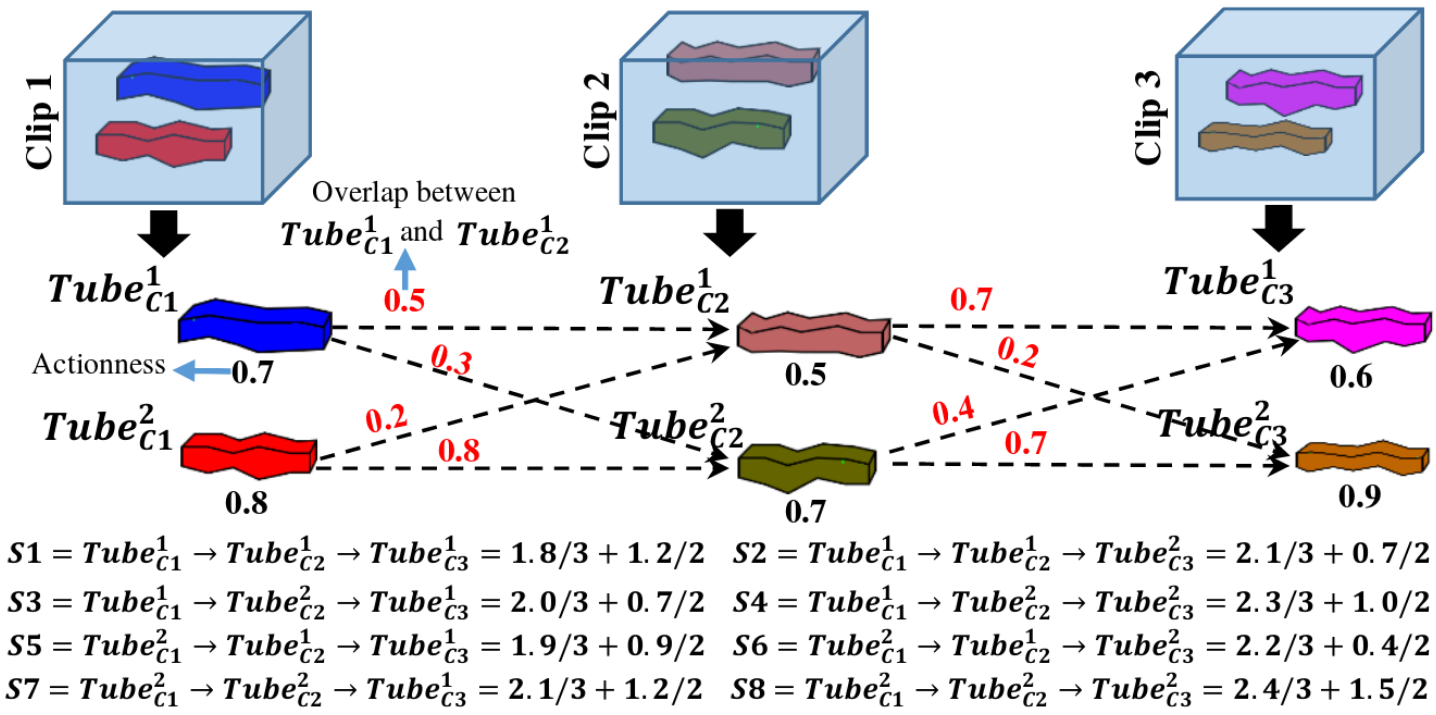
\includegraphics[scale=0.225]{connection_algo}
  \caption{An example of calculating connection score for 3 random TOIs}
  \label{fig:connection_algo}
\end{figure}

For every possible combination of TOIs we calculate their score as show in figure \ref{fig:connection_algo}.
The above approach, however, needs too much memory for all needed calculations, so a memory usage  problem is
appeared. The reason is, for every new video segments we propose \textit{k TOIs} (16 during training and 150 during validation).
As a result, for a small video seperated in  \textbf{5 segments}, we need to calculate
\textbf{  16\textsuperscript{5}  combinations at least}. \par

In order to deal with this problem, we create a greedy algorithm in order to find the candidates tubes. Inituitively, this algorithm after
a new video segment keeps tubes with score higher than a threshold, and deletes the rest.
So, we don't need to calculate combinations with very low score. This algorithm is described below:
\begin{enumerate}
\item Firstly, initialize empty lists for the final tubes, their scores, active tubes, their overlapping sum and actioness sum where:
  \begin{itemize}
  \item Final tubes list contains all tubes which are the most possible to contain an action, and their score list contains their
    corresponding scores.
  \item Active tubes list contains all tubes that will be match with the new TOIs. Their overlapping sum list and actioness sum list
    contain their sums in order to avoid calculating then for each loop. 
  \end{itemize}
Also, we initialize threshold equal to 0.5 .
\item For the first video segment, we add all the TOIs to both active tubes and final tubes. Their scores are only their actioness because
  there are no tubes for calculating their overlapping score. So, we set their overlaping sum equal to 0.
\item For each next video, firstly we calculate their overlapping score with each active tube. Then, we empty active tubes, overlapping
  sum and actioness score lists.  For each new tube that has score higher than the threshold we add to final tubes and to active tubes.
\item If the number of active tubes is higher than a threshold (1000 in our situation), we set the threshold equal to the score of
  the 100th higher score. On top of that, we update the final tubes list, removing all tubes that have score lower than the threshold.
\item After that, we add in active tubes, the current video segment's proposed TOIs. Also their actioness scores in actioness sum list and
  zero values in corrensponding positions in overlaps sum list (such as in the 1st step).
\item We repeat the previous 3 steps until there is no video segment left.
\end{enumerate}

\section{Some results}
For both TPN approaches we kept the same connecting algorithm. We experiment mainly in the value of the updating threshold.

\subsection{JHMDB dataset}
As we know, this dataset uses trimmed videos. So alongside with the previous algorithm, we experiment using the same
approach without step 5.
\subsection{UCF dataset}

\end{document}
